\chapter{结合主动学习和半监督学习的视频压缩}

在本章中我们将介绍如何结合主动学习核半监督学习来进行视频压缩。我们使
用PSNR来衡量图像压缩的质量。

同之前的视频着色和压
缩\cite{learning-to-compress-images,colorization-using-optimization}一
样,我们将使用$YUV$空间。其中$Y$是灰度通道,而$U$和$V$则是存储颜色的色
度通道。我们将独立地预测$U$和$V$两个通道的值。
在\cite{learning-to-compress-images} 中,用于表示一个像素点的特征包括空
间信息和局部的纹理信息。我们经过实验发现局部纹理信息对于预测颜色值来说
并没有什么帮助,因此,我们仅使用空间信息和灰度值来表达每个像素点的特
征。

对于一个一共有$\ell$帧,每一帧有$n$个像素点的视频。首先,我们在第一帧上
应用第 \ref{chap:semi-supervised-learning} 章中所描述的半监督学习算法来
学习一个模型,然后用这个模型来预测该帧以及后续一些帧的颜色值。当PSNR值
低于一定阈值时,我们会重新训练一个模型。半监督学习的过程需要对一一个$m
\times m$的稠密矩阵求逆,这是非常大的计算量。为了减轻计算负担,Chen et
al. \cite{learning-to-compress-images} 建议使用 NCut
\cite{learning-a-classification-model-for-segmentation} 将图像分割成一
些小区域,然后使用 {\em super-pixel} 来表示每个小区域,并在这些小区域
中随机地选择像素点来参与计算。不过 NCut 本身就是一个很耗时的算法。在我
们的工作中,我们采用直接将图像划分为小方格个形式,从而避免了复杂的分割
算法。在我们实验的实验中,我们将小方格的个数定位 2000 个。然后我们会随
机地从每个小方格选取一个像素点,这样总共会有 2000 个像素点,然后我们会
在这些像素点上构造 4-邻接图。

一旦构造好了邻接图,我们就可以应用主动学习的算法来选取最具有代表性的像
素点。视频压缩的质量会随着所选的像素点的数量变化而变化,选的点越多,质
量就会越高。另一方面,选择更多的点会降低压缩比。由于图是在 2000 个点上
构造的,因此最多可以选择 2000 个点。解码的过程就是应用半监督学习算法来
学习一个模型,并用它来预测灰度像素点的颜色值。

考虑到视频数据在时间上的平滑性,一个视频的帧之间不会变化太快,从某一帧
训练出来的颜色模型可以直接被应用到接下来的一些帧上而不会造成太多的视觉
上的差异。在我们的实验中,我们设置一个阈
值 $\Delta_{PSNR}$。令 $PSNR^{*}$表示用于训练模型的那一帧的着色质量,我
们将一直使用该模型来预测后续的帧,知道得到的 PSNR 值低
于$PSNR^{*}-\Delta_{PSNR}$为止,此时我们将会重新训练一个模型。因为着色
模型是在单个帧上训练出来的,因此我们把这种方法叫做``单帧模型''(Single
Frame Model, SFM)。最终我们会得到一些着色模型 $SFM_1, \cdots,
SFM_k$,着色模型说对应的那些帧称作关键帧,用 $KF_1, \cdots, KF_k$ 表
示。

为了利用视频在时间上的局部性,我们按照下述步骤进一步扩展我们的方法。为
特征空间添加新的一维表示时间的分量$t$,主动学习和半监督学习都将在这个新
的特种空间中进行。与原来使用单帧来训练模型的方法不同,这次我们将同时使
用多个帧来学习,具体地说,我们将关键帧分割为一个一个的时间区间,保证单
个区间内的帧之间的差别不是太大,然后一个区间内的数个关键帧将被用来训练
一个着色模型。我们将这种方法称作多帧模型 (Multiple Frame Model, MFM)。
类似地,我们会得到一系列的着色模型 $MFM_1, \cdots, MFM_l$。需要注意的
是,$MFM_i$仅仅用于预测它所在的那个时间区间内的帧。

\begin{figure*}[t]
  \center \subfigure[原始帧]{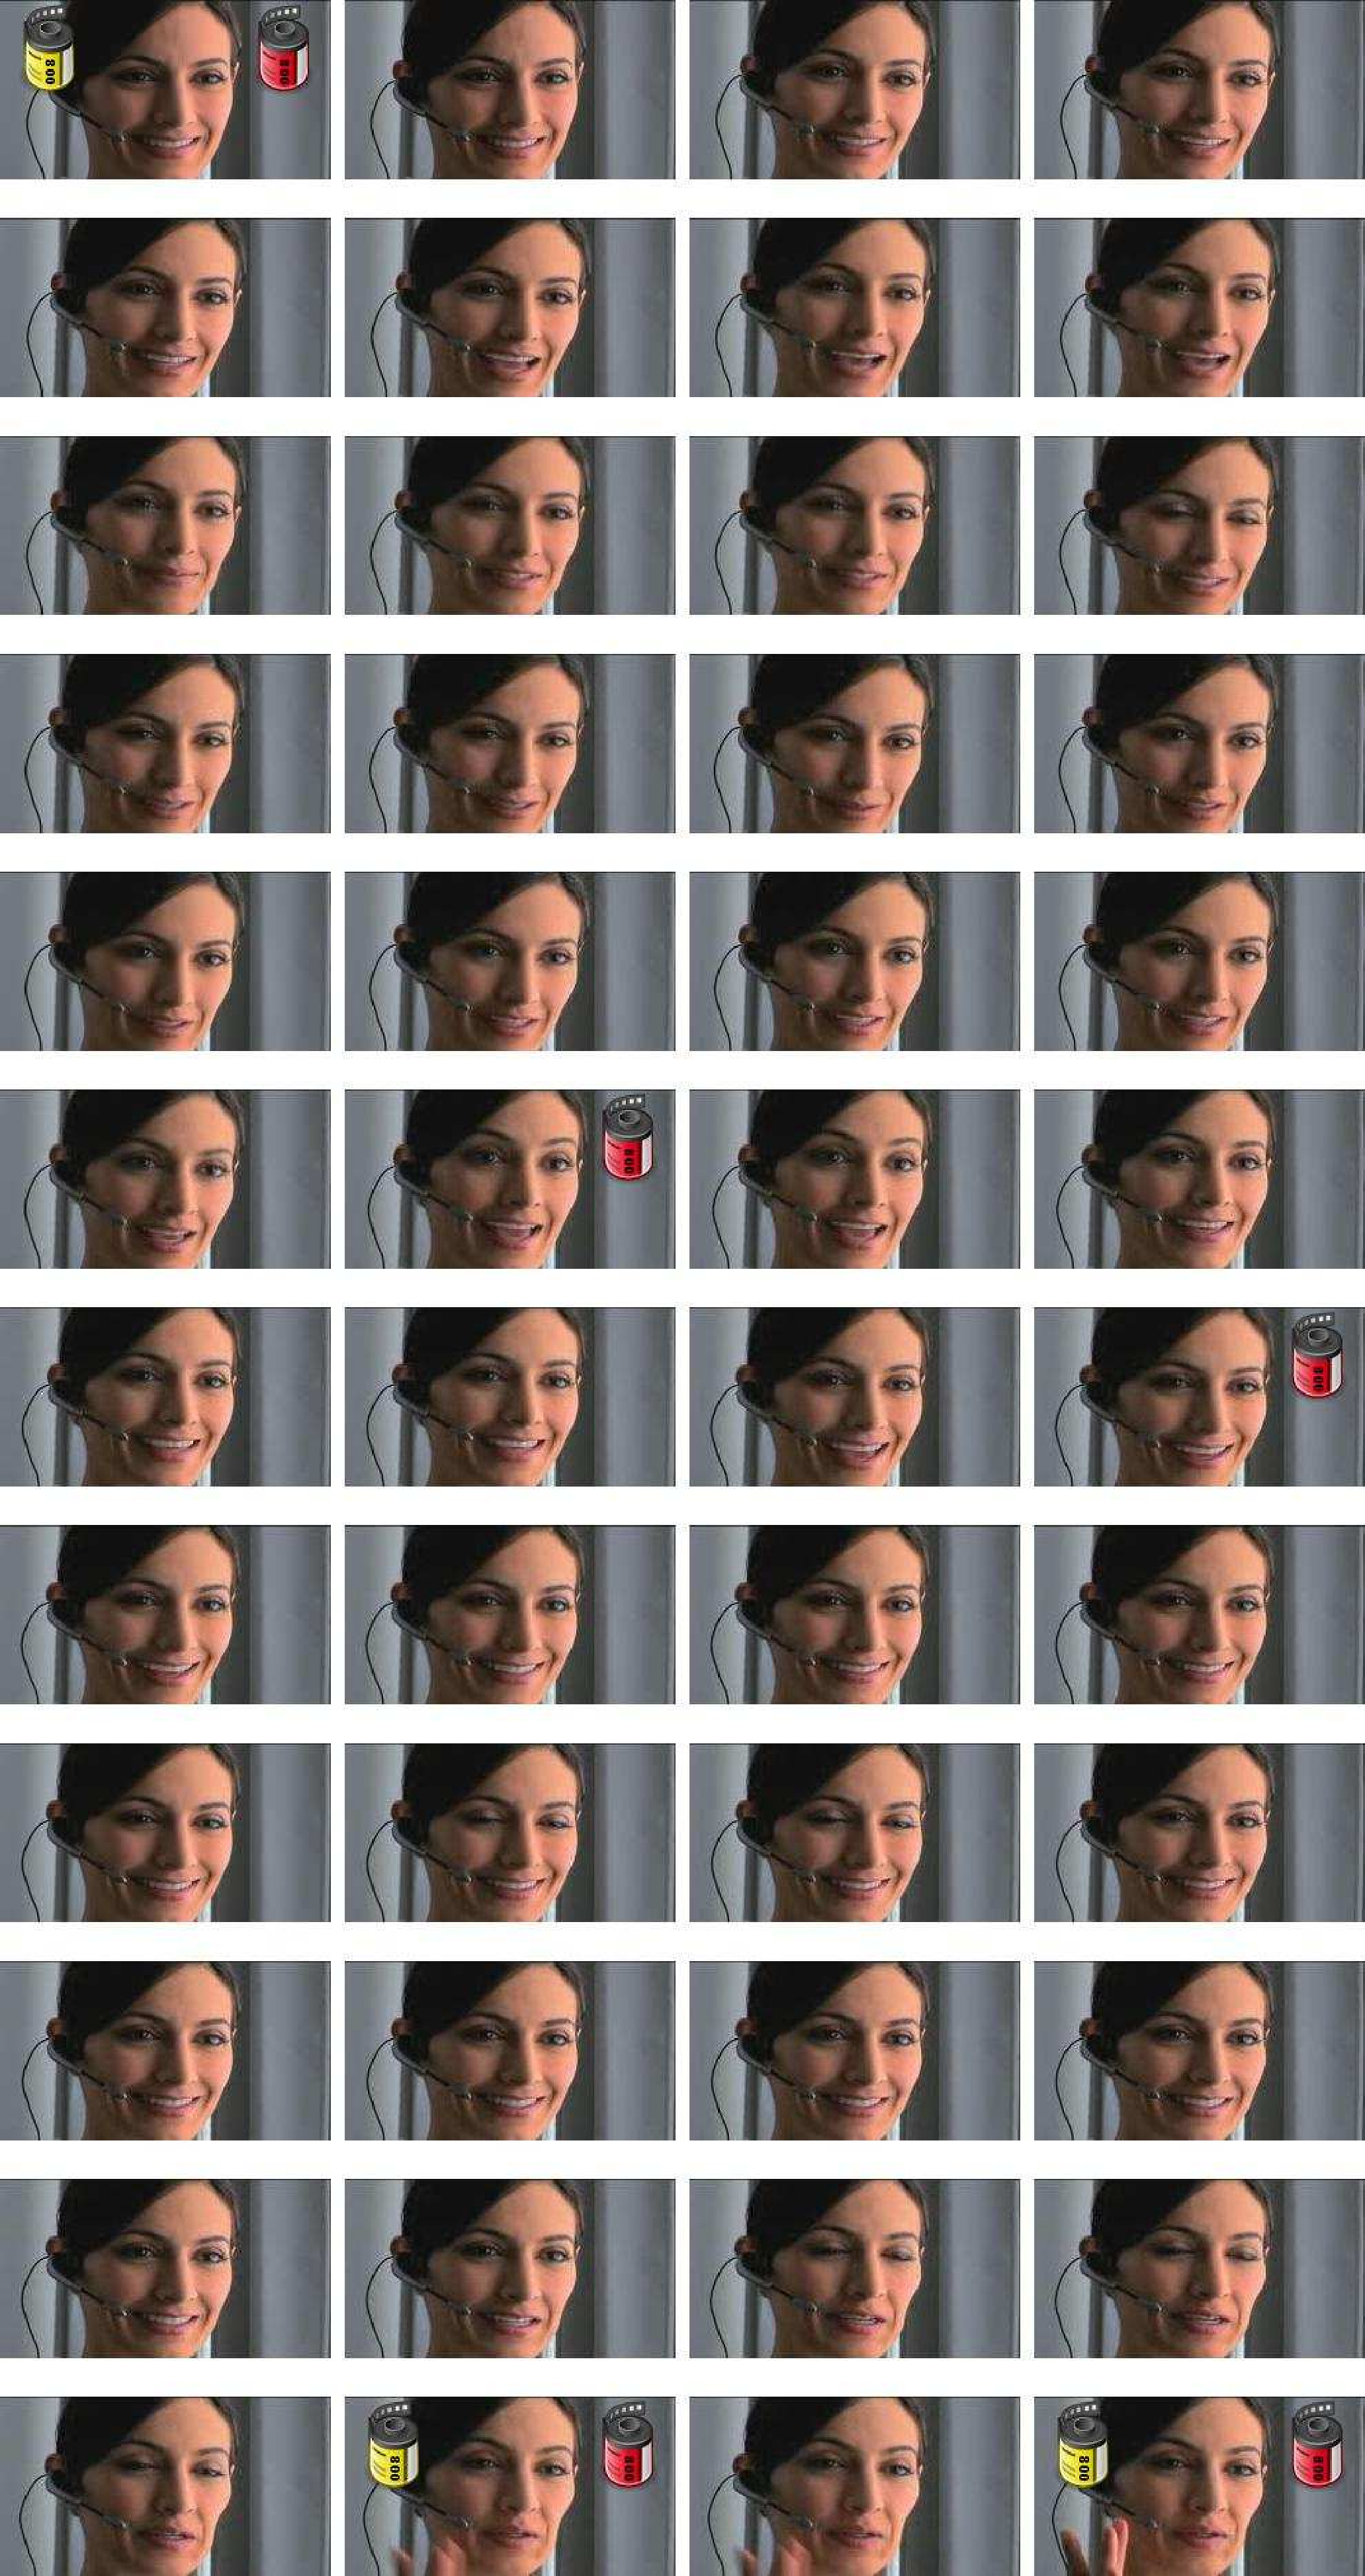
\includegraphics[width=.4\linewidth]{images/telemarket-frames}}
  \hspace{4mm} \subfigure[着色帧]{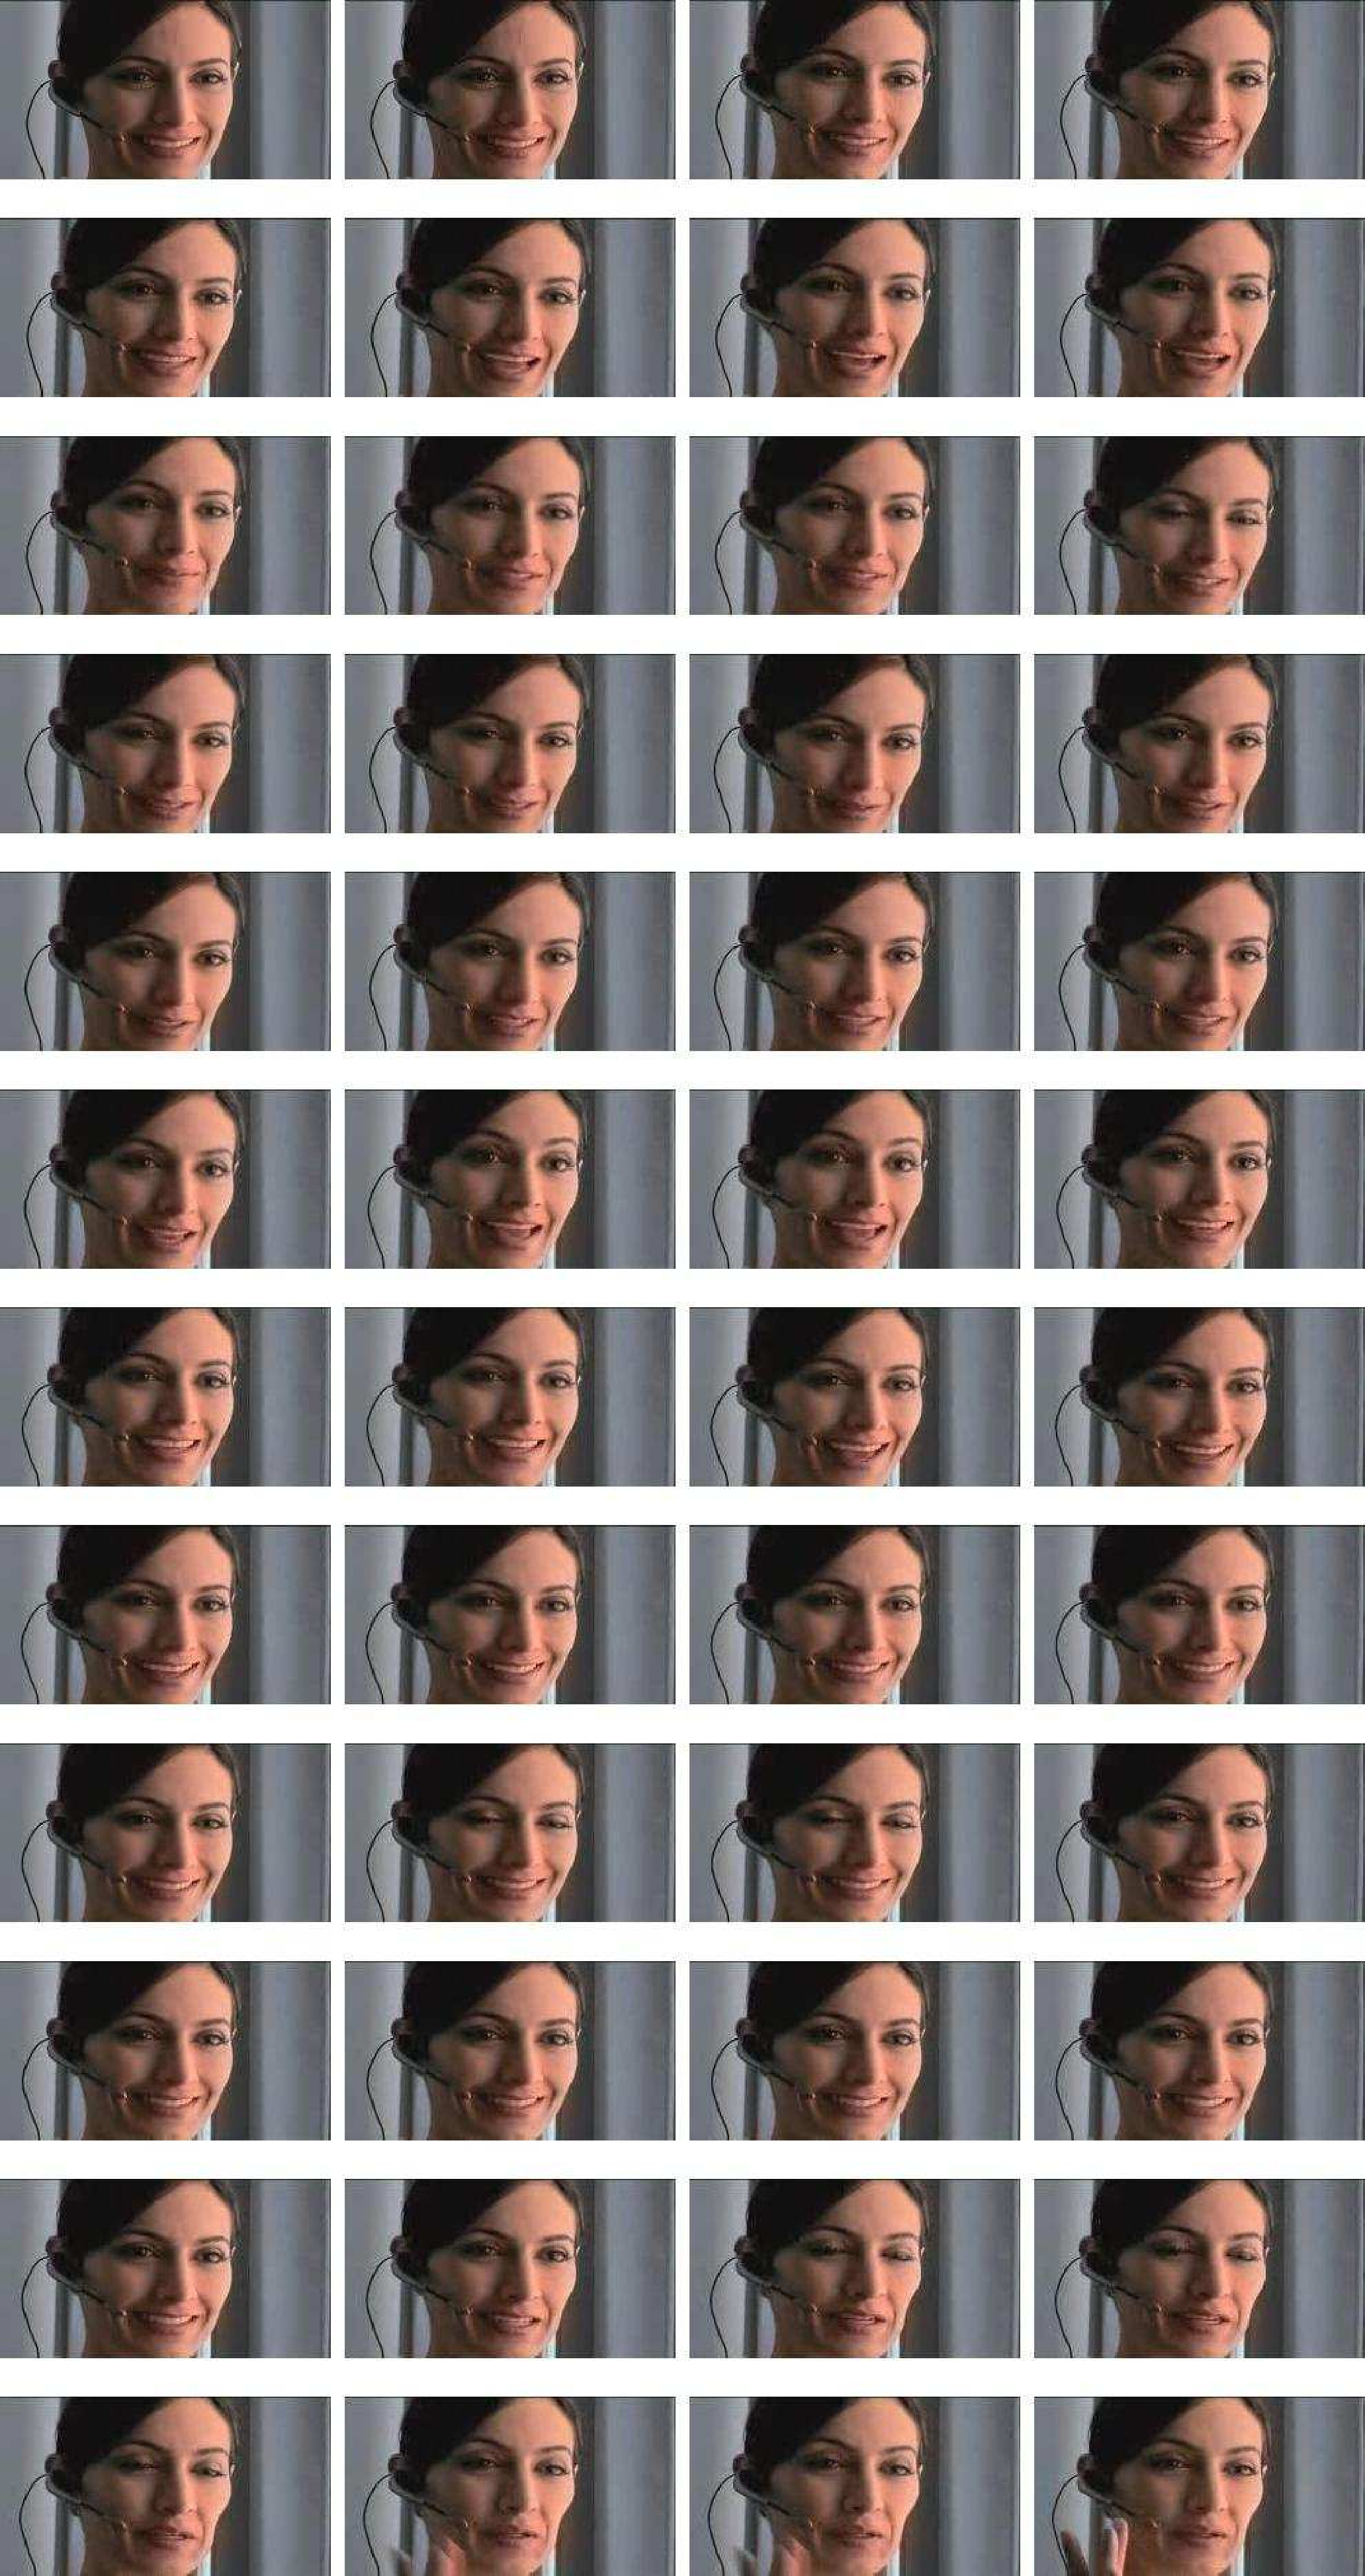
\includegraphics[width=.4\linewidth]{images/telemarket-rcv}}
\caption{接线员视频的初始 48 帧。我们的方法重新训练模型的帧由黄色的胶
  卷图标标出,Cheng 的方法重新训练模型的帧则由红色胶卷图标标出。}
\label{fig:telemarket}
\end{figure*}


\begin{table*}[t]
  \centering \scriptsize
  \caption{视频压缩结果。 cr 表示压缩比(compression ratio)}
  \label{tab:more-example}
  \begin{tabular}{|l|c|c|c|c|c|c|c|c|c|c|}
    \hline
    video & orig. size & gray. size & \multicolumn{2}{|c|}{Cheng's approach} & \multicolumn{2}{|c|}{SFM} & \multicolumn{2}{|c|}{MFM} & \multicolumn{2}{|c|}{MPEG-4} \\
    \cline{4-11}
    & & & cr & PSNR & cr & PSNR & cr & PSNR & cr & PSNR \\
    \hline
    claire & 463452 & 44556 & 10.48\% & 29.7 & 10.48\% & 35.2 & 10.65\% & \textbf{35.6} & 10.48\% & 35.0 \\
    \hline
    miss-america & 229148 & 17082 & 11.82\% & 35.7 & 11.82\% & 36.4 & 10.60\% & \textbf{37.0} & 11.09\% & 36.0 \\
    \hline
    akiyo & 226780 & 26588 & 12.61\% & 28.3 & 12.61\% & 33.0 & 13.31\% & 33.6 & 12.77\% & \textbf{33.9} \\
    \hline
    suzie & 466278 & 98926 & 34.08\% & 38.5 & 33.23\% & 40.3 & 30.61\% & \textbf{41.1} & 39.29\% & 40.7 \\
    \hline
    mother-daughter & 466836 & 117302 & 28.98\% & 38.2 & 28.55\% & 40.4 & 27.70\% & \textbf{41.2} & 27.54\% & 39.9 \\
    \hline
  \end{tabular}
\end{table*}

